\chapter{System Evaluation}
\label{Milan}


% Evaluation method and calibration 
% Detector Cal 
% System Cal 
% System evaluation 
% hard ware issues 

% New Event Recon (killed_LRF, FilteredSpectrum, Normalisation)
% New Linearity software (3 methods) 
In this chapter the use of the \acrshort{INSERT} scanner is outlined. The calibration procedures and experimental methods explored in this chapter are used to evaluated the system performance. The outcome of this investigation resulted in the implementation of new data processing methods. 

\section{Introduction}
The following experiments were carried out at \acrlong{HSR} (\acrshort{HSR}), in collaboration with Politecnico di Milano (POLIMI). The system was transported and installed in the nuclear medicine department in order to carry out experiments with radioisotopes such as Technetium-99m. The experiments were carried out using the BULMA software provided by Mediso Ltd (Budapest). The software was designed to operate the system and acquired the raw data from experiments. The raw data was processed and calibrated using the BULMA INSERT-GUI package along with existing system data. 
\paragraph{}
These experiments set out to acquire the first phantom images from the \acrshort{INSERT} system, and in order to achieve this the system was first evaluated and calibrated. The count-rate and energy resolution were determined and the system corrections and calibrations for these parameters where carried out at Polimi. The calibration procedures required to correct for event and image reconstruction are outlined here.
\paragraph{}
The calibration procedure was developed on a single detector head system \cite{8069508}, and was tested in this investigation for the first time on the complete \acrshort{INSERT} scanner. This investigation aimed to determine the effectiveness of the proposed calibration method, and evaluate the systems performance and imaging capabilities. The calibration involves two stages: the detector calibration and the system calibration. The event reconstruction was corrected through the detector calibration procedure; a standard linearity and uniformity correction was performed. The image reconstruction was carried out using the geometric and sensitivity information obtained by the system calibration.

%\section{Methods}
\section{Detector Calibration}
Uniformity and linearity are subject to position and time variations and so we must calibrate each detector regularly. The detector calibration is carried out by collecting uniformity and linearity data from each detector head. The uniformity of a given detector head is determined by the intensity variation across a planar acquisition. The uniformity is subject to spatial variations in the crystal properties such as, stopping power and number of emitted scintillation photons. Linearity is a measure of location dependent spatial distortion. This measured by reproducing a known linear geometry.
\paragraph{}
The uniformity data is collected by performing a flood scan of a single point source (1 MBq of $^{99m}Tc$) located in the centre of the scanner \acrshort{FOV}. The uniformity scan was carried out without the collimator attached; consequently short scans are required due to the high counts. The uniformity scans were collected once and used to correct for uniformity in the subsequent phantom acquisitions. 
\paragraph{}
The linearity distortion in a given detector was measured by acquiring data from a planar phantom (4 MBq of $^{99m}Tc$) mounted a set of parallel line collimators (figure \ref{fig:LinColl}). Two collimator scans are carried out on each head; measuring the distortion in the X and Y direction respectively. The phantom attached to the linearity collimator only covers a single detector head and so each unit was scanned individually. 40, four minute scans were required to collect the complete set of X and Y linearity data. 

\begin{figure}[!t]
%\vspace{-0.2cm}
\centering
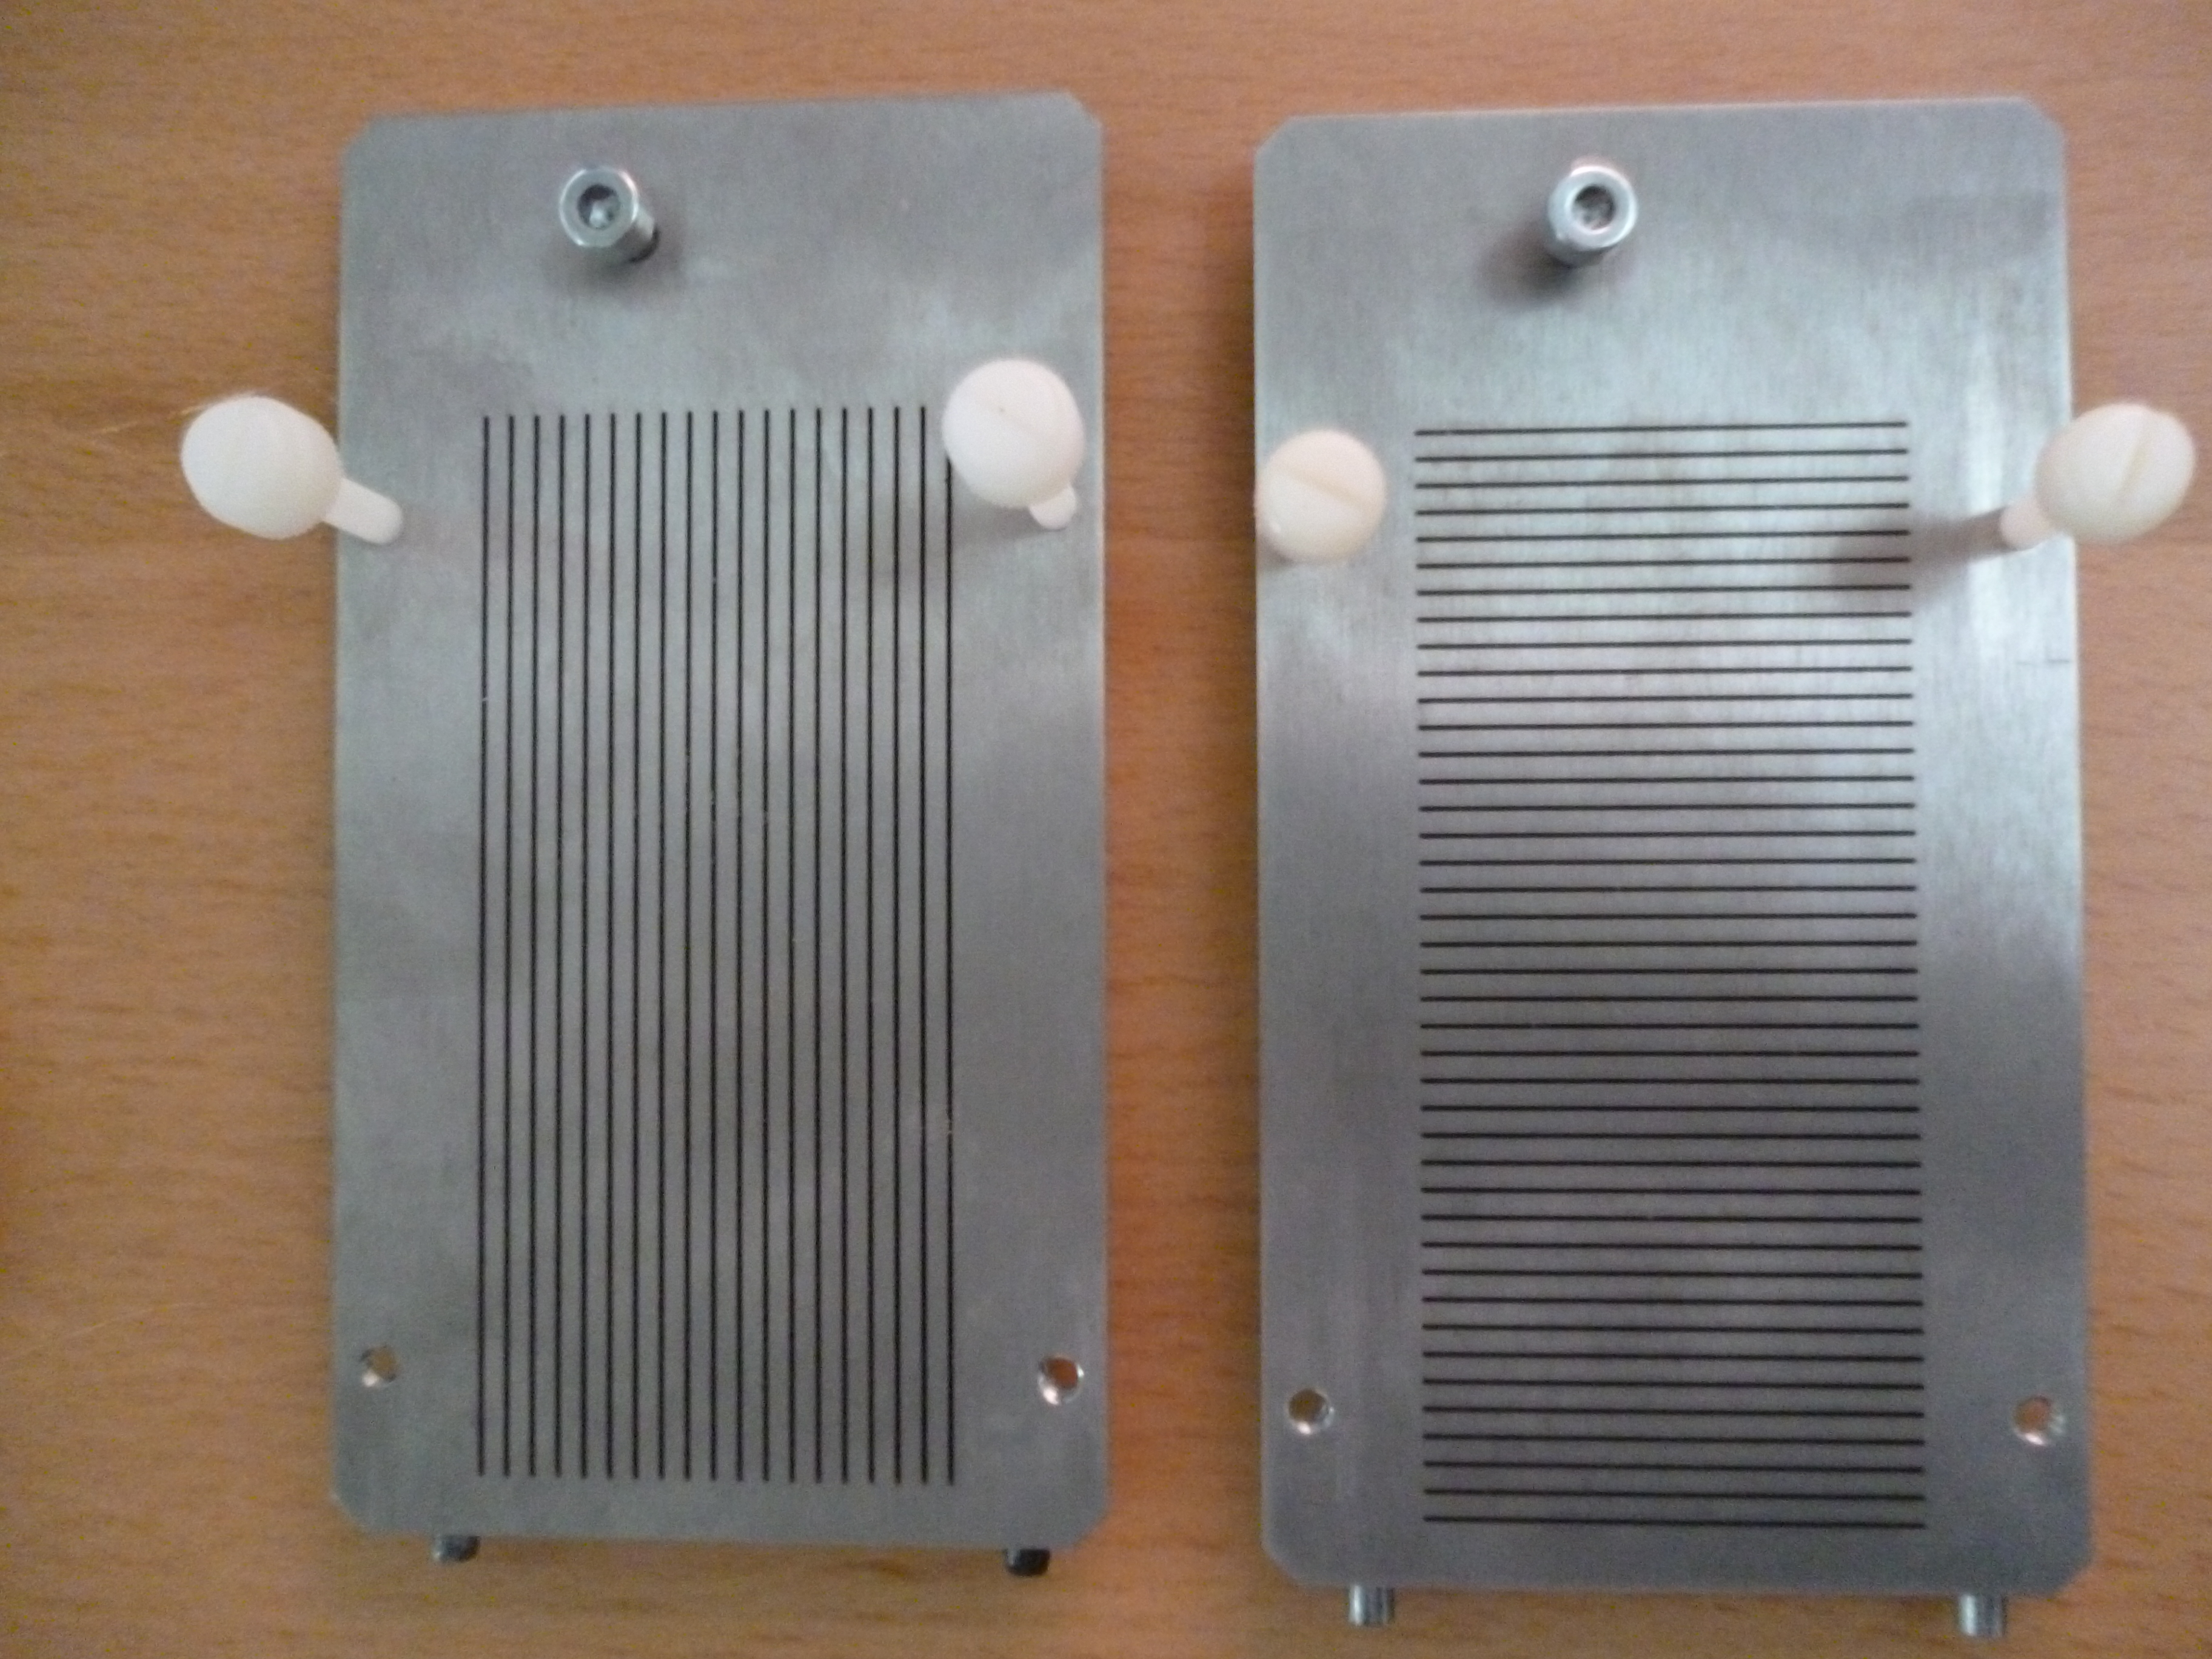
\includegraphics[width=3.6in]{figures/P1020277.JPG}

    \caption{The parallel line collimators used to carry out the linearity calibration.} \label{fig:LinColl}
%\vspace{-0.2cm}
\end{figure}

\subsection{Detector Calibration Software}
The resulting data is processed using the BULMA software. The uniformity and linearity data is used to produce a set of transformation maps which are applied during the planar event reconstruction. As discussed previously the planar event reconstruction is carried out in a two step method; a \acrshort{COM} reconstruction is used to initialise an \acrshort{ML} reconstruction. Part of the \acrshort{ML} algorithm is the modelling of the detectors spatial response, the aforementioned \acrshort{LRF}. The BULMA software included existing \acrshort{LRF} data for the system, however it was found that this data was incorrect for the current system. The uniformity flood was used to produce a new set of \acrshort{LRF} models, which were incorporated in the event reconstruction.
\paragraph{}
The \acrshort{LRF}, uniformity, and the X/Y linearity data are input into the BULMA software alongside the raw uncorrected phantom data. The X and Y data are firstly reconstructed to produce two planar images of linear bands. The software uses active contour splines to identify the data bands. The resulting X and Y splines are combined to produce a grid of crossing control points; the linearity map is created. The photopeak of the total phantom data is determined and an initial reconstruction is found using the \acrshort{LRF}. The linearity map crossing points mark out positions to determine the local energy spectra; these produce a local, position-dependent, energy filter. The energy at each pixel position in the phantom reconstruction are calculated and matched to the local energy map. Correcting for the local energy peaks produces a planar reconstruction corrected for energy and linearity. The uniformity data is reconstructed in the same way to create the uniformity map. The phantom reconstruction is multiplied by the inverse of the uniformity map to correct each pixel. The final result is a corrected planar image, ready for image reconstruction. 

%\subsection{Uniformity}
%\subsection{Linearity} 

\section{System Calibration}
The image reconstruction algorithm requires information of the systems geometry and sensitivity \cite{Beque2003CharacterizationGeometry}. The system calibration acquires this information through two experiments. Each experiment is carried out with the collimator fitted. The data from each experiment produces corrections, which are applied to the planar images during image reconstruction. 
 \paragraph{}
The geometric calibration has been established and tested previously on a single detector unit \cite{8340862}. The geometric data is acquired from a series of scans of capillary phantoms. The capillaries have 1 mm diameter and are filled with 10 MBq of $^{99m}Tc$. Two experiments are set up to acquire the axial and trans-axial geometry of the system. 
\paragraph{}
\textbf{Axial Orientation:} The capillaries were aligned with the axial direction of the scanner. The capillaries are held on a rotating stage and positioned at four locations with the \acrshort{FOV}. The positions are separated by $90\degree$ and lie at radii of 25, 50, 75 and 100 mm. From these positions, the capillaries are rotated about the z axis of the scanner. The capillaries are scanned for two minutes at 30 positions; rotating by $12\degree$ until $360\degree$ is covered. 
\paragraph{}
\textbf{Trans-axial Orientation:} similarly the capillaries were placed along the trans-axial plane and rotated about the z axes. Five capillaries are at positions, $ 0, \pm 5, \pm 10 $ cm from the centre of the bore. Due to time constraints these capillaries were only scanned for five positions.
\paragraph{}
The sensitivity calibration required data with a planar phantom, $10 * 10 * 0.5$ cm, filled with 50 MBq of $^{99m}Tc$. The phantom was place in front of each detector head and scanned individually (figure \ref{fig:georCal}). The phantom covered the whole collimator \acrshort{FOV}, the resulting flood acquisition gave a measure of uniformity variation due to the collimator geometry. 

\begin{figure}[!t]
%\vspace{-0.2cm}
\centering
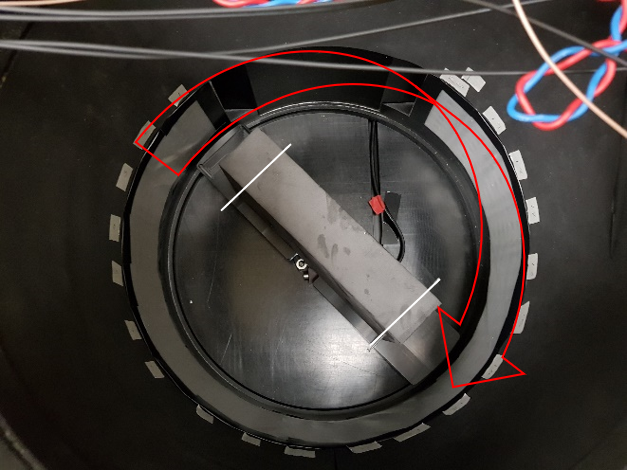
\includegraphics[width=3.4in]{figures/geoCal.png}
\caption{The capillaries are placed on a rotating stage and scanned at each position at the centre of a given detector face.}
\label{fig:georCal}
%\vspace{-0.2cm}
\end{figure}

\subsection{System Calibration Software}
The data collected from the system calibration undergoes planar event reconstruction and detector calibration as described above. The resulting data was analysed in MATLAB.
\paragraph{}
The geometric data was used to measure 3 system parameters of the collimator \cite{TianyuMa2007DeterminationMicroPET}. The tilt and twist angles, and mechanical shifts were determined by modelling the variation in position and size of the capillary data. The location of each capillary is measures with a Gaussian model by taking measurements along its length. The variation in position as a function of radial position of the axial capillaries is known as the mechanical shift in the collimator. The variation of position along the length of a trans-axial capillary is known as the twist angle. Finally the variation in position as a function of radial position of the trans-axial capillaries gives us a measure of the tilt angle. 
\paragraph{}
The reconstructed sensitivity profiles gave a measure of count variation across the whole collimator \cite{Accorsi2008DerivationCollimation}. The sensitivity variation as a function of sampling angle of the aperture was modelled. Each profile was fitted using equation (\ref{sens_model}), where $\phi$ is the sampling angle, $G_{\sigma}(\phi)$ is a Gaussian function. The summation is carried out over all mini-slits $i$ for each collimator section $j$. The model is used to correct for sensitivity variation in the planar projection data. 

\begin{equation}
%\vspace{-0.2cm}
\label{sens_model}
S_{j}(\phi) = \sum_{i} G_{\sigma}(\phi) \ast A_{i,j} \cos^{p}{\phi} + b_{j}(\phi)
%\vspace{-0.2cm}
\end{equation}

\section{Results}
The calibration procedures were used to carry out the correct image reconstruction of the phantom data, the use of this data will be shown in chapter \ref{IEEE}. However, the data collected in these experiments were also used to assess the system performance and to determine system properties such as resolution and stability. 

\subsection{Detector Calibration}
 The uniformity scans were used to quickly assess the condition of each detector. The initial assessment revealed the presence of faulty channels in some detector heads. A faulty channel would produce a high number of false counts which resulted in a hot spot; drowning out the healthy channels and giving further false counts to neighbouring channels. The solution to this was to turn off, or `kill', the offending channels and leave a single dead channel in its place. The dead channel left a large gap in the projection data; event reconstruction was carried out but detector calibration was not possible. The \acrshort{LRF} provided a solution to this problem as it gave the spatial response for each individual channel. The killed channels were therefore modelled as a such in the \acrshort{LRF} data. This was achieved by building an \acrshort{LRF} model with the 'killed' uniformity data. This allowed the \acrshort{MLEM} reconstruction to model the missing data and interpolate events from neighbouring channels. The modified reconstruction significantly reduced the data gap left by the faulty channel.
 \paragraph{}
 The detectors were found to have higher linearity towards the centre, with large distortions towards the crystal edges, hot spots and killed channels. The \acrshort{LRF} fix allowed for linearity correction in killed channels. However, severe distortion required manual intervention when creating the linearity maps. The software was amended to include a manual fix for the active contour splines; in which the path of the contour is chosen by hand. Figure \ref{fig:LRFCorr} shows the use of BULMA software with \acrshort{LRF} correction to remove the failed detector channel. 

\begin{figure}[!t]
%\vspace{-0.2cm}
\centering
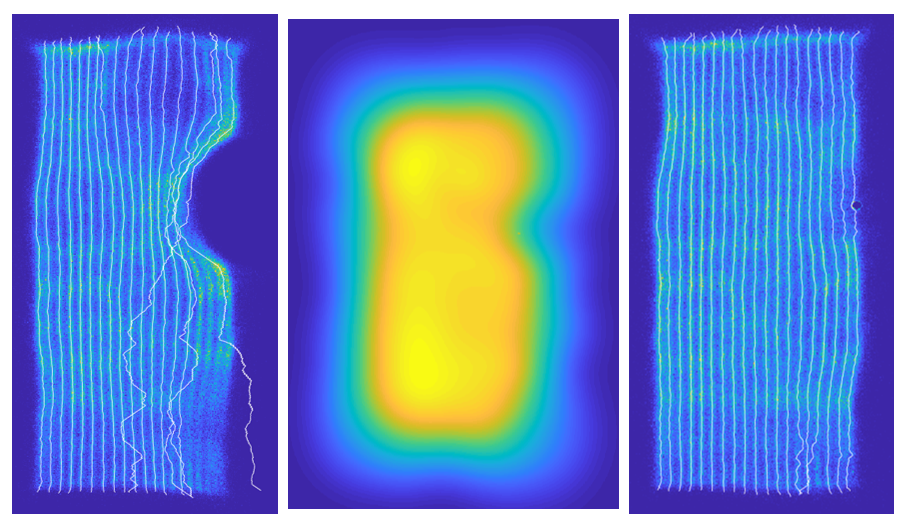
\includegraphics[width=3.4in]{figures/LRF_transform.png}
\caption{The failed channel causes an error in the spline model. By introducing the appropriate LRF model (centre) the failed channel is modelled and the correct splines are found.}
\label{fig:LRFCorr}
%\vspace{-0.2cm}
\end{figure}

\subsection{System Calibration}
The 3 parametric angles determined by the geometric calibration were each measured to give a distortion close to zero. This suggests negligible distortion, therefore a stable collimator set up. This result was expected as the geometric calibration was established on a single detector head system; in which the position and orientation of the collimator was unknown with regards to the source. The complete system has a fixed known geometry, and so the relative position of the phantom to all 20 collimator units is constant. 
\paragraph{}
The capillary acquisitions served a secondary purpose; investigating the system resolution. The reconstructed planar projections provided a measure of the scanner head resolution (combined detector and collimator resolutions), where as the final image reconstructions gave a measure of image resolution. 
\paragraph{}
The axial resolution was measured by calculating the \acrlong{FWHM} (\acrshort{FWHM}) of the Gaussian fitted to the trans axial capillary data. Figure \ref{fig:AxialRes} shows the result of measurements. As expected the resolution degrades as the source is moved further from the detector head. As stated previously, only 5 detectors were measured due to time constraints. These results show a slight degradation in resolution compared to previous measurements; this is likely due to ageing hardware. 

\begin{figure}[!t]
%\vspace{-0.2cm}
\centering
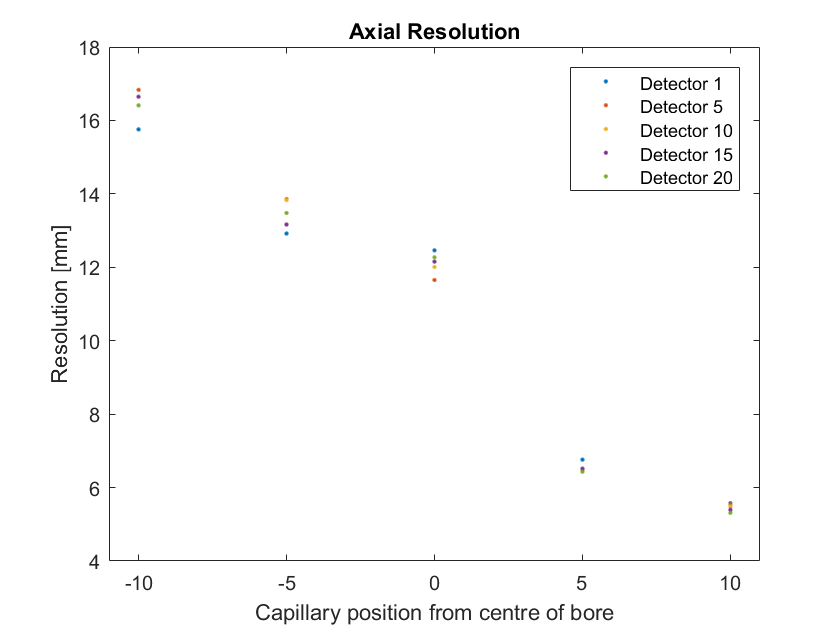
\includegraphics[width=3.4in]{figures/AxialRes.png}
\caption{The transaxial resolution measured from capillaries placed at various locations within the INSERT bore.}
\label{fig:AxialRes}
%\vspace{-0.2cm}
\end{figure}

The sensitivity calibration resulted in 20 planar projections; giving a measure of count variation for each detector. By inspecting a slice through the data with the sensitivity model a series of sensitivity profiles. Fig. \ref{fig:sensprof} shows examples of sensitivity profiles for two different collimator sections and the corresponding fits. This models were fitted for every slit section across the length of the collimator. Through the model a measure of count variation was determined and compared against the expected geometry of the system. Reconstruction was then corrected for the count variation for each slit section. 

\begin{figure}[!t]
%\vspace{-0.2cm}
\centering
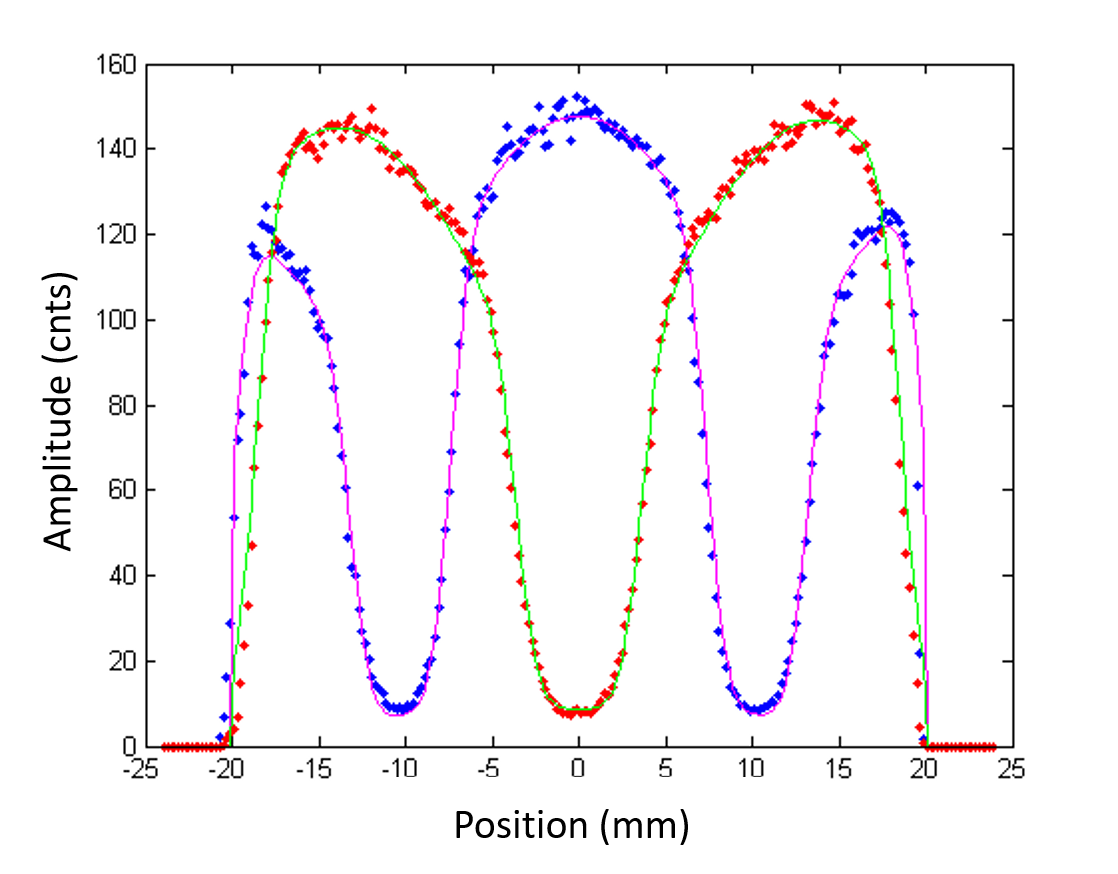
\includegraphics[width=3.4in]{figures/sns_prof.png}
\caption{Sensitivity profiles for two collimator sections and fitted analytical functions.}
\label{fig:sensprof}
%\vspace{-0.2cm}
\end{figure}

\section{Discussion}
The experiments carried out here were the first use of the calibration and acquisition procedures on the complete system. The goal of this study was to acquire the first phantom images and assess the system performance, however, we also look critically at the procedures and software used in the system. When compared to initial studies \cite{8432104} we found a degradation in system performance; this is due to ageing of the components and stress on the system from regular use. Despite this we were able to use the system extensively and collect a large quantity of data. The results of the investigation lead to changes in software, processing methods and calibration. 
\paragraph{}
The detector calibration revealed major issues when using the aged system. The channel instability resulted in data lost and false counts. The hot spots caused by faulty channels reduced the quality of the acquire data, requiring data channels to be removed completely from acquisition. Constant faulty channels could be switched off and accounted for with the \acrshort{LRF} models. Figures \ref{fig:killchan} and \ref{fig:killcorr} demonstrate the corrections possible when using the adapted \acrshort{LRF} reconstruction. 

\begin{figure}[!tbp]
  \centering
  \subfloat[Detector with a failed channel at (3.7,4.7)]{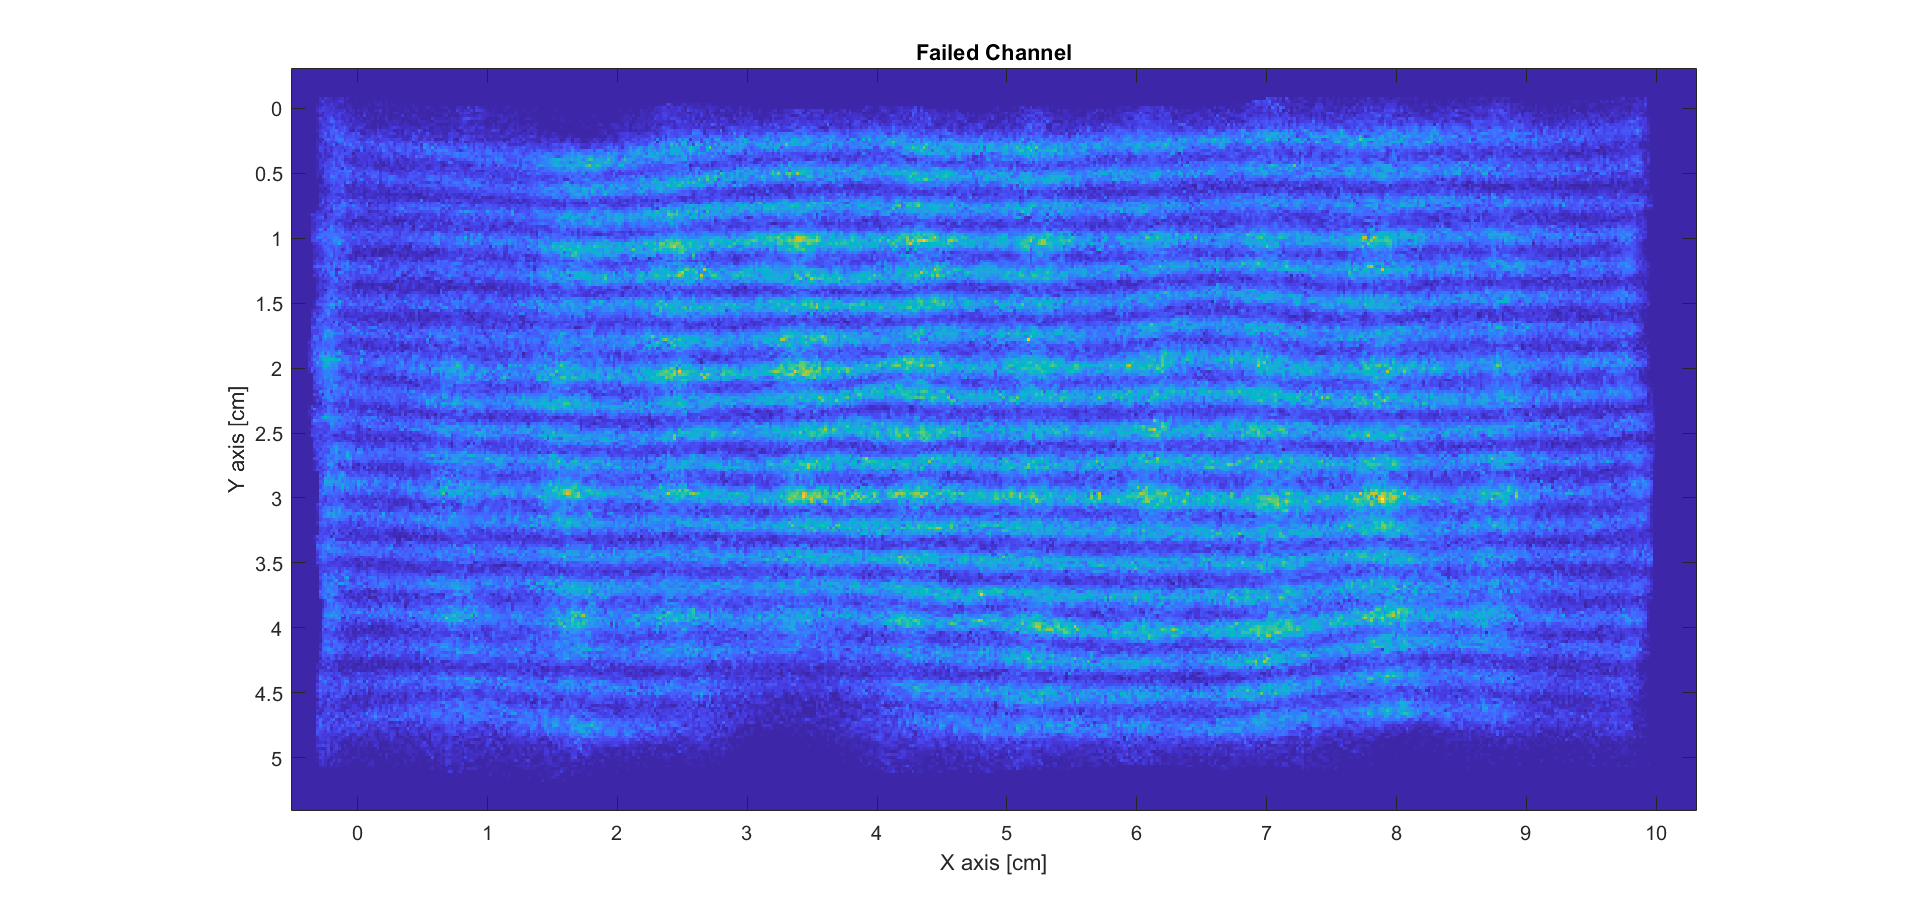
\includegraphics[width=1\textwidth]{figures/FailedChnl.png}\label{fig:killchan}}
  \hfill
  \subfloat[Complete calibration and reconstruction procedure has corrected this projection ]{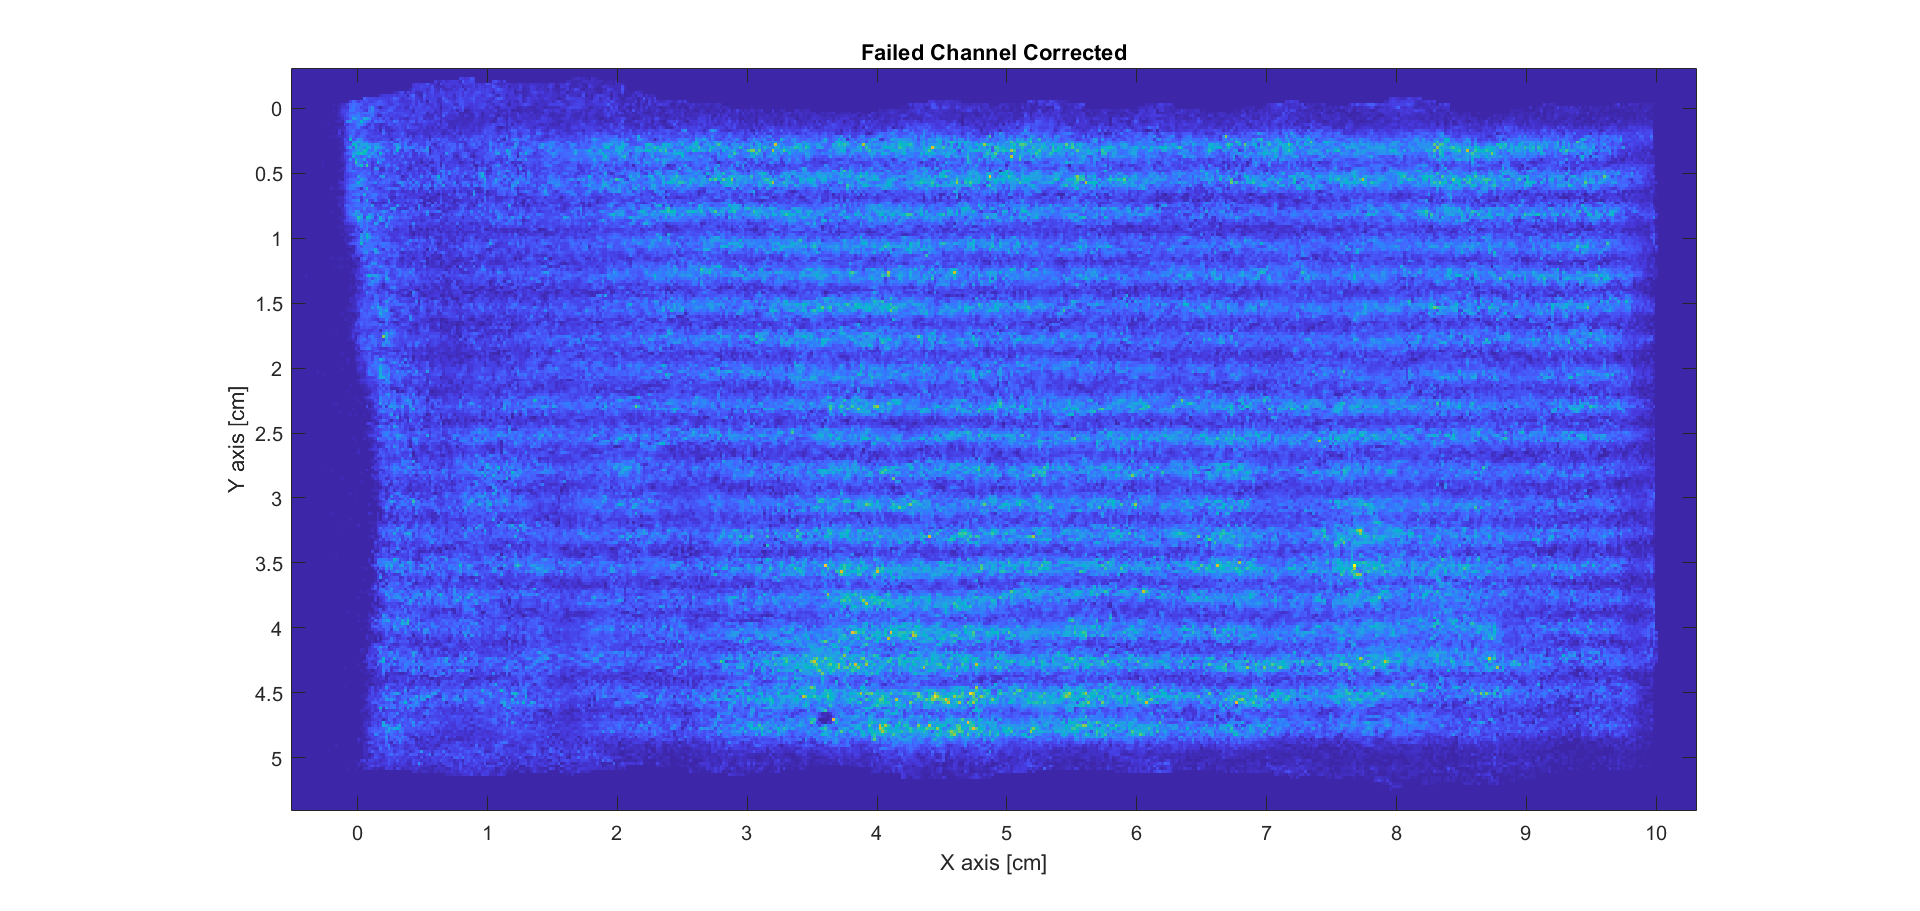
\includegraphics[width=1\textwidth]{figures/FailedCorr.png}\label{fig:killcorr}}
  \caption{The \acrshort{LRF} and calibration procedures are used here to correct the distortion in the projection data.}
\end{figure}

The \acrshort{LRF} is successful in accounting for faulty channels, however it is only effective when correcting for single channels. If several channels are missing in one place, there will not be enough neighbouring data to interpolate the missing area. When faced with large areas of detectors failure we can make use of dual acquisition. The two acquisition positions allow a larger area of data to be collected. By rotating the detector view we can retrieve angles from whole detector failure.
\paragraph{}
The linearity acquisitions made use of the BULMA software to produce correction maps. We found that large linearity distortion required manual intervention. This was time consuming as 40 data sets required manual correction. The acquisition of linearity data required individual scans were also time consuming; combined, the acquisition and processing of the linearity correction maps took five days. As we have seen the stability of the detectors can lead to failure in the calibration. In order to repeat the calibration regularly we require an improved process which can be completed quickly and effectively. When the correction maps were applied to the acquisition data it was found that the edges of the data were truncated. We investigated the BULMA software, but the cause of this truncation was not found. This truncation lead to loss of data and errors in the final image reconstructions. The current software is only designed for the given calibration and acquisition procedure. In order to implement a new calibration procedure and remove the truncation issues we propose the development of a new calibration software; chapter \ref{Linearity} will cover the implementation of this software. 
\paragraph{}
The results of the geometric calibration were found to be constant; as the system geometry is fixed and known, we can calculate the parameters without calibration. The geometric calibration was designed for a single detector system and therefore no longer required in the complete system; we propose to remove this step in future investigations. In future experiments we set out to change the system and detector calibration procedures. 

\section{Conclusion}
The calibration data was collected successfully and the results will be shown in chapter \ref{IEEE}. However the time taken to acquire and process this data was not acceptable for regular use. A new software and calibration process will be designed and implemented to improve use of the system. In the next chapter we will see how the phantom data is affected by the new software.
\paragraph{}
The stability of the system is a concern as faulty detectors and variability reduces the quality of the data. Although detector failure was accounted for, a further investigation is required to determine the extend of detector instability. The possibility of replacing faulty components would resolve many issues. Until this time we continue to implement procedures to collect and process data quickly and  produce correct images.
